Tutti gli utenti, a prescindere dal livello, possono consultare i dati raccolti dal nodo (cfr. \ref{dati-raccolti}) in tre sezioni principali:
\begin{itemize}[noitemsep,nolistsep]
    \item Calibrazioni (o Capture)
    \item Stack
    \item Detection
\end{itemize}

Nella sezione corrente verranno trattate insieme le prime due (cfr. figure \ref{fig:calibrazioni} e \ref{fig:stack}), dal momento che sono analoghe eccetto per i dati.

\subsection{Visualizzazione dati raccolti} \label{capture-struct}

Sia le calibrazioni che gli stack sono organizzati in una struttura tabellare analoga a quella delle cartelle sul nodo (cfr. \ref{dati-raccolti}). La \textbf{prima tabella} contiene l'elenco dei \textbf{giorni}, dieci per pagina, e il numero delle calibrazioni o degli stack di quel giorno. La \textbf{seconda tabella} mostra invece le calibrazioni o gli stack del giorno selezionato sulla prima tabella, anche in questo caso dieci per pagina. Ciascuna riga contiene \textbf{nome della calibrazione/stack}, l'\textbf{ora} in cui è stata catturata l'immagine e due pulsanti, \textbf{Anteprima} e \textbf{Download} (cfr. figura \ref{fig:capture-table}). Sotto le tabelle è mostrata l'\textbf{ultima immagine rilevata} e relativa didascalia.

\begin{wrapfigure}{r}{0.3\textwidth}
    \vspace{-30pt}
    
\includegraphics[width=0.3\textwidth]{images/toggle-button.jpg}
    \vspace{-30pt}
\end{wrapfigure}
Il pulsante \textbf{Download} permette di scaricare il \textbf{file FITS} dell'immagine ed è sempre abilitato.
Il pulsante \textbf{Anteprima} mostra invece a schermo in una \textbf{finestra modale} l'immagine convertita in \textbf{PNG} in modo da poterla visualizzare (cfr. figura \ref{fig:capture-preview}). Si noti che questo pulsante è disabilitato di default: per porterlo abilitare è necessario attivare il \textbf{\emph{toggle button}} in alto a destra. Una volta attivato, l'utente dovrà aspettare una manciata di secondi, dal momento che il server si occupa di convertire tutte e dieci le immagini (cfr. sezione \ref{elaborazione-dati-capture}) che vengono poi mandate al client in codifica \emph{Base64} e memorizzate in locale. Il \emph{toggle button} è stato pensato per non appesantire l'esperienza dell'utente nello scorrere le pagine della tabella con inutili caricamenti.
Per implementare questa funzionalità si è fatto un largo uso dell'implementazione server-side di \textbf{DataTables}.

\begin{figure}[H]
    \begin{center}
    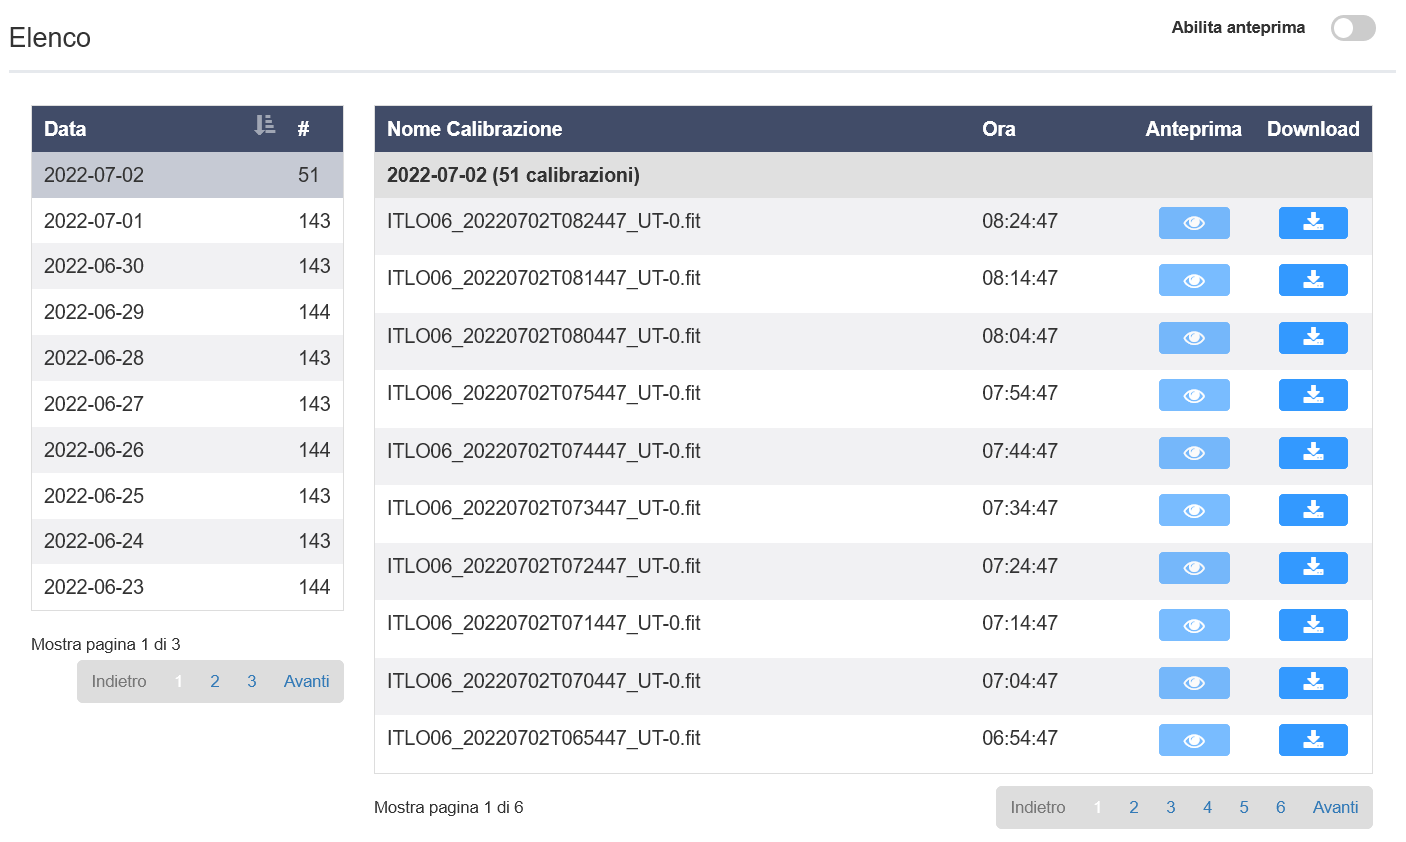
\includegraphics[width=\textwidth]{images/captures-table.png}
    \caption{Visualizzazione elenco calibrazioni di un giorno.}
    \label{fig:capture-table}
    \end{center}
\end{figure}
\vspace{-24pt}
\begin{figure}[H]
    \begin{center}
    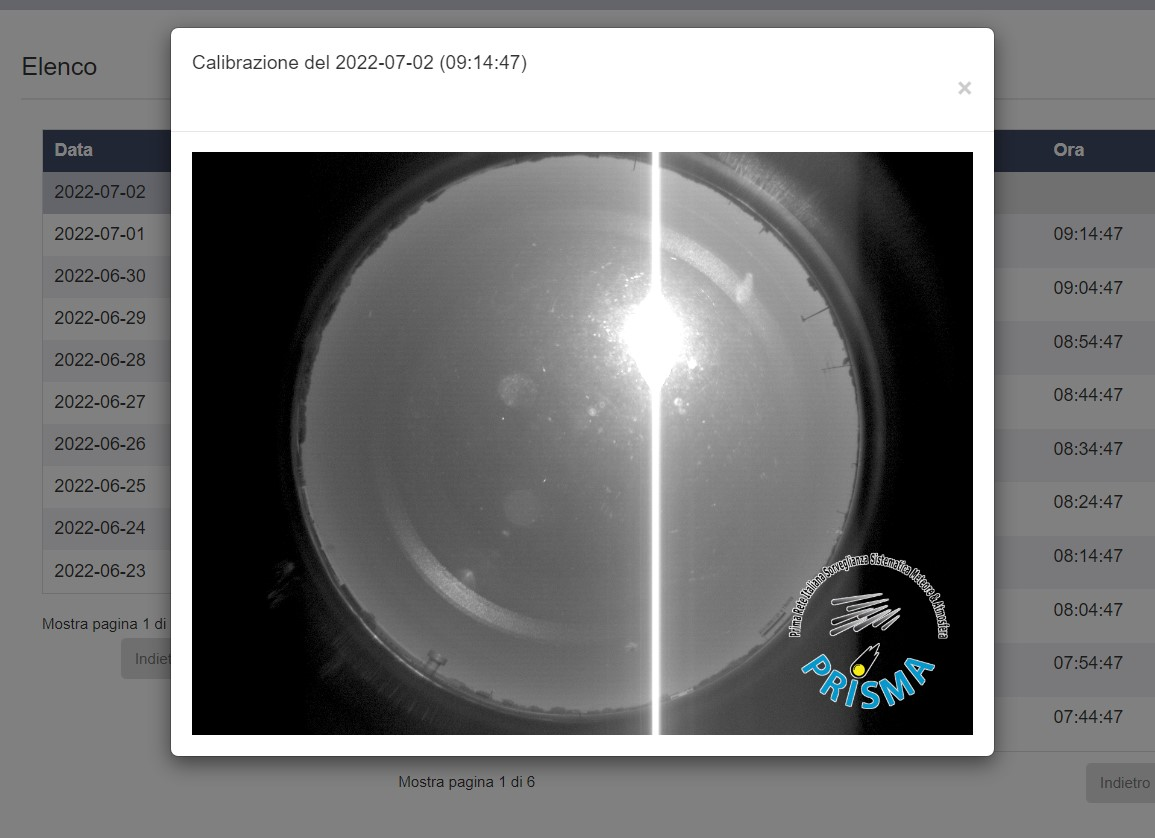
\includegraphics[width=\textwidth]{images/capture-preview.jpg}
    \caption{Anteprima di una calibrazione.}
    \label{fig:capture-preview}
    \end{center}
    
\end{figure}

\subsection{Elaborazione dei dati server-side} \label{elaborazione-dati-capture}

Quando l'utente abilita il \emph{toggle button}, oppure cambia pagina quando è attivo, il server si occupa di elaborare ciascuno dei dieci file consultabili in modo da rendere disponibile la visualizzazione dell'immagine lato client: il browser altrimenti non avrebbe modo di renderizzare il formato FITS.

L'elaborazione di ciascun file attraversa tre stadi:

\begin{enumerate}
    \item \textbf{Conversione in PNG}: il file FITS viene convertito in formato PNG mediante il software \textbf{fitspng} (cfr. sezione \ref{software});
    \begin{verbatim}
        fitspng -o <output_file> <input_file>
    \end{verbatim}
    \item \textbf{Watermarking}: all'immagine convertita viene aggiunto il logo del progetto PRISMA in basso a destra, servendosi di \textbf{ImageMagick} (cfr. sezione \ref{software});
    \begin{verbatim}
        composite -gravity SouthEast <logo> \ 
            <input_image> <output_image>
    \end{verbatim}
    \item \textbf{Conversione in \emph{Base64}}: il file ottenuto viene infine codificato in \emph{Base64} (cfr. listing \ref{lst:base64-coding}) .
\end{enumerate}

Si noti che tutti i file vengono temporaneamente salvati in una cartella di webroot e poi, una volta codificati in \emph{Base64} vengono eliminati per non occupare ulteriore spazio.

\begin{lstlisting}[style=PHP,caption={Metodo PHP per codificare i file in \emph{Base64}.},captionpos=b,label={lst:base64-coding}]
    // Encode image to base64
    public static function encodeCapture($path) {
        if (!file_exists($path)) {
            return "";
        }
        $data = file_get_contents($path);
        $base64 = 'data:image/png;base64,' . 
            base64_encode($data);
        return $base64;
    }
\end{lstlisting}

\begin{figure}[H]
    \begin{center}
    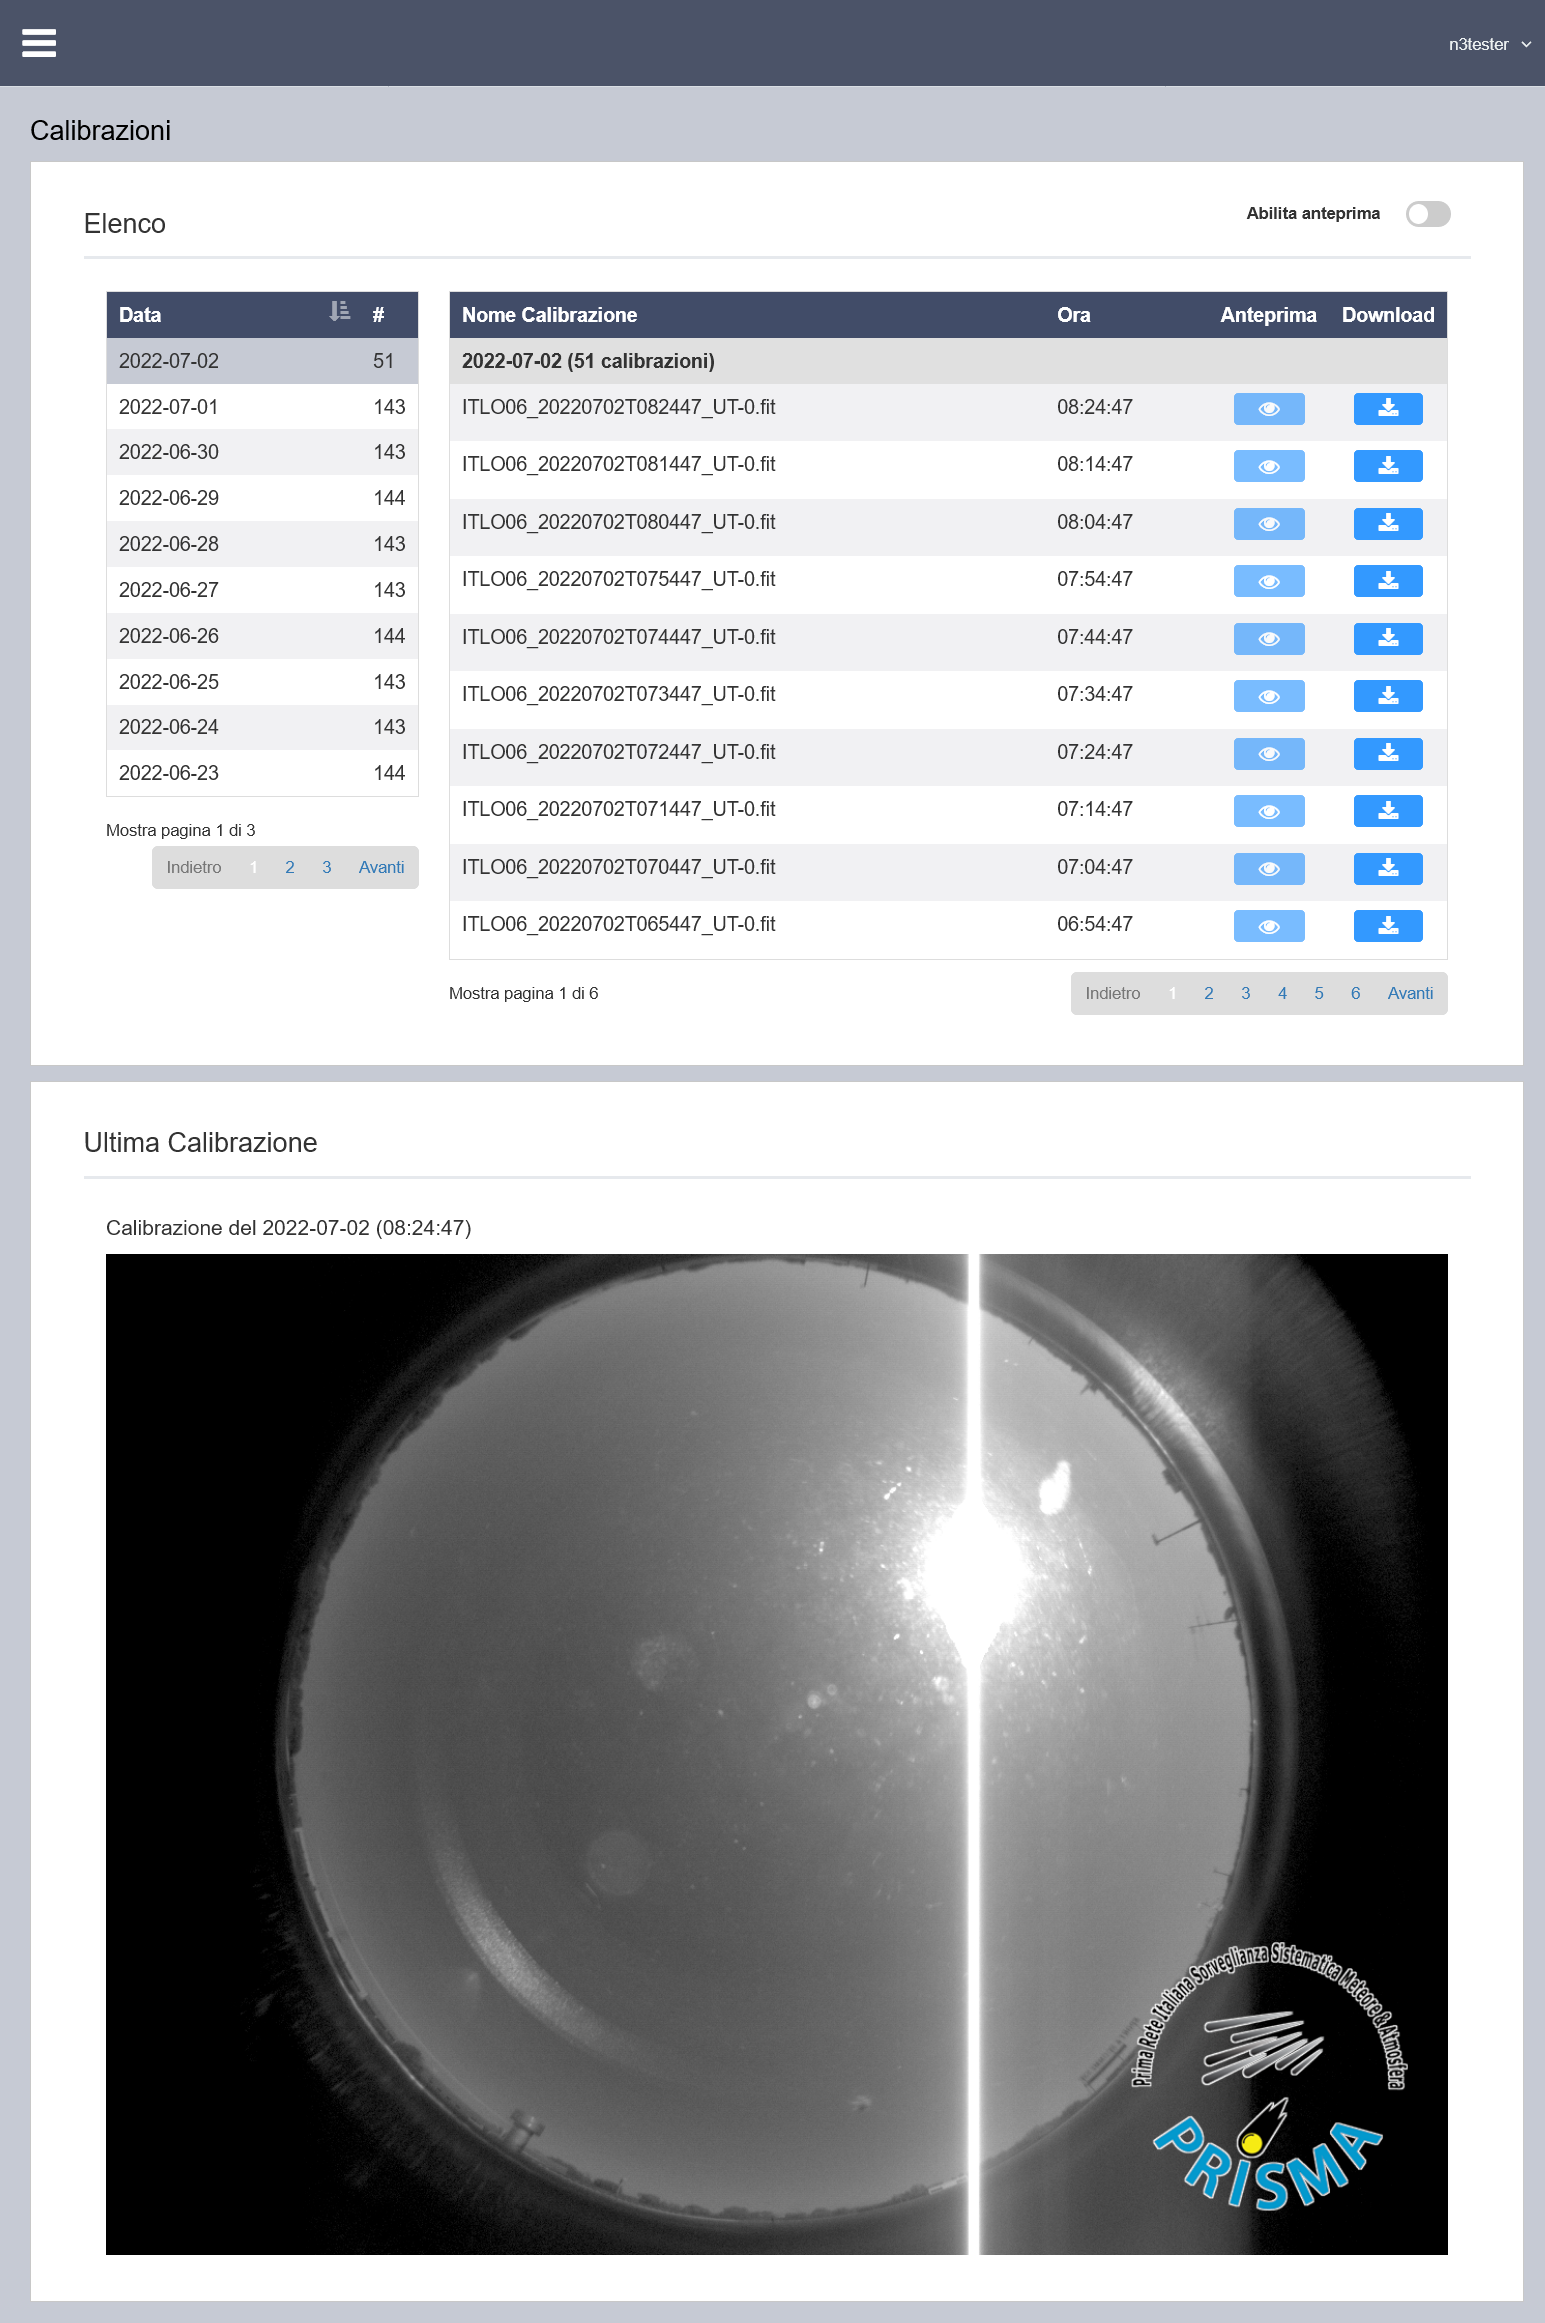
\includegraphics[width=\textwidth]{images/full-captures.png}
    \caption{Sezione \emph{Calibrazioni}.}
    \label{fig:calibrazioni}
    \end{center}
\end{figure}

\begin{figure}[H]
    \begin{center}
    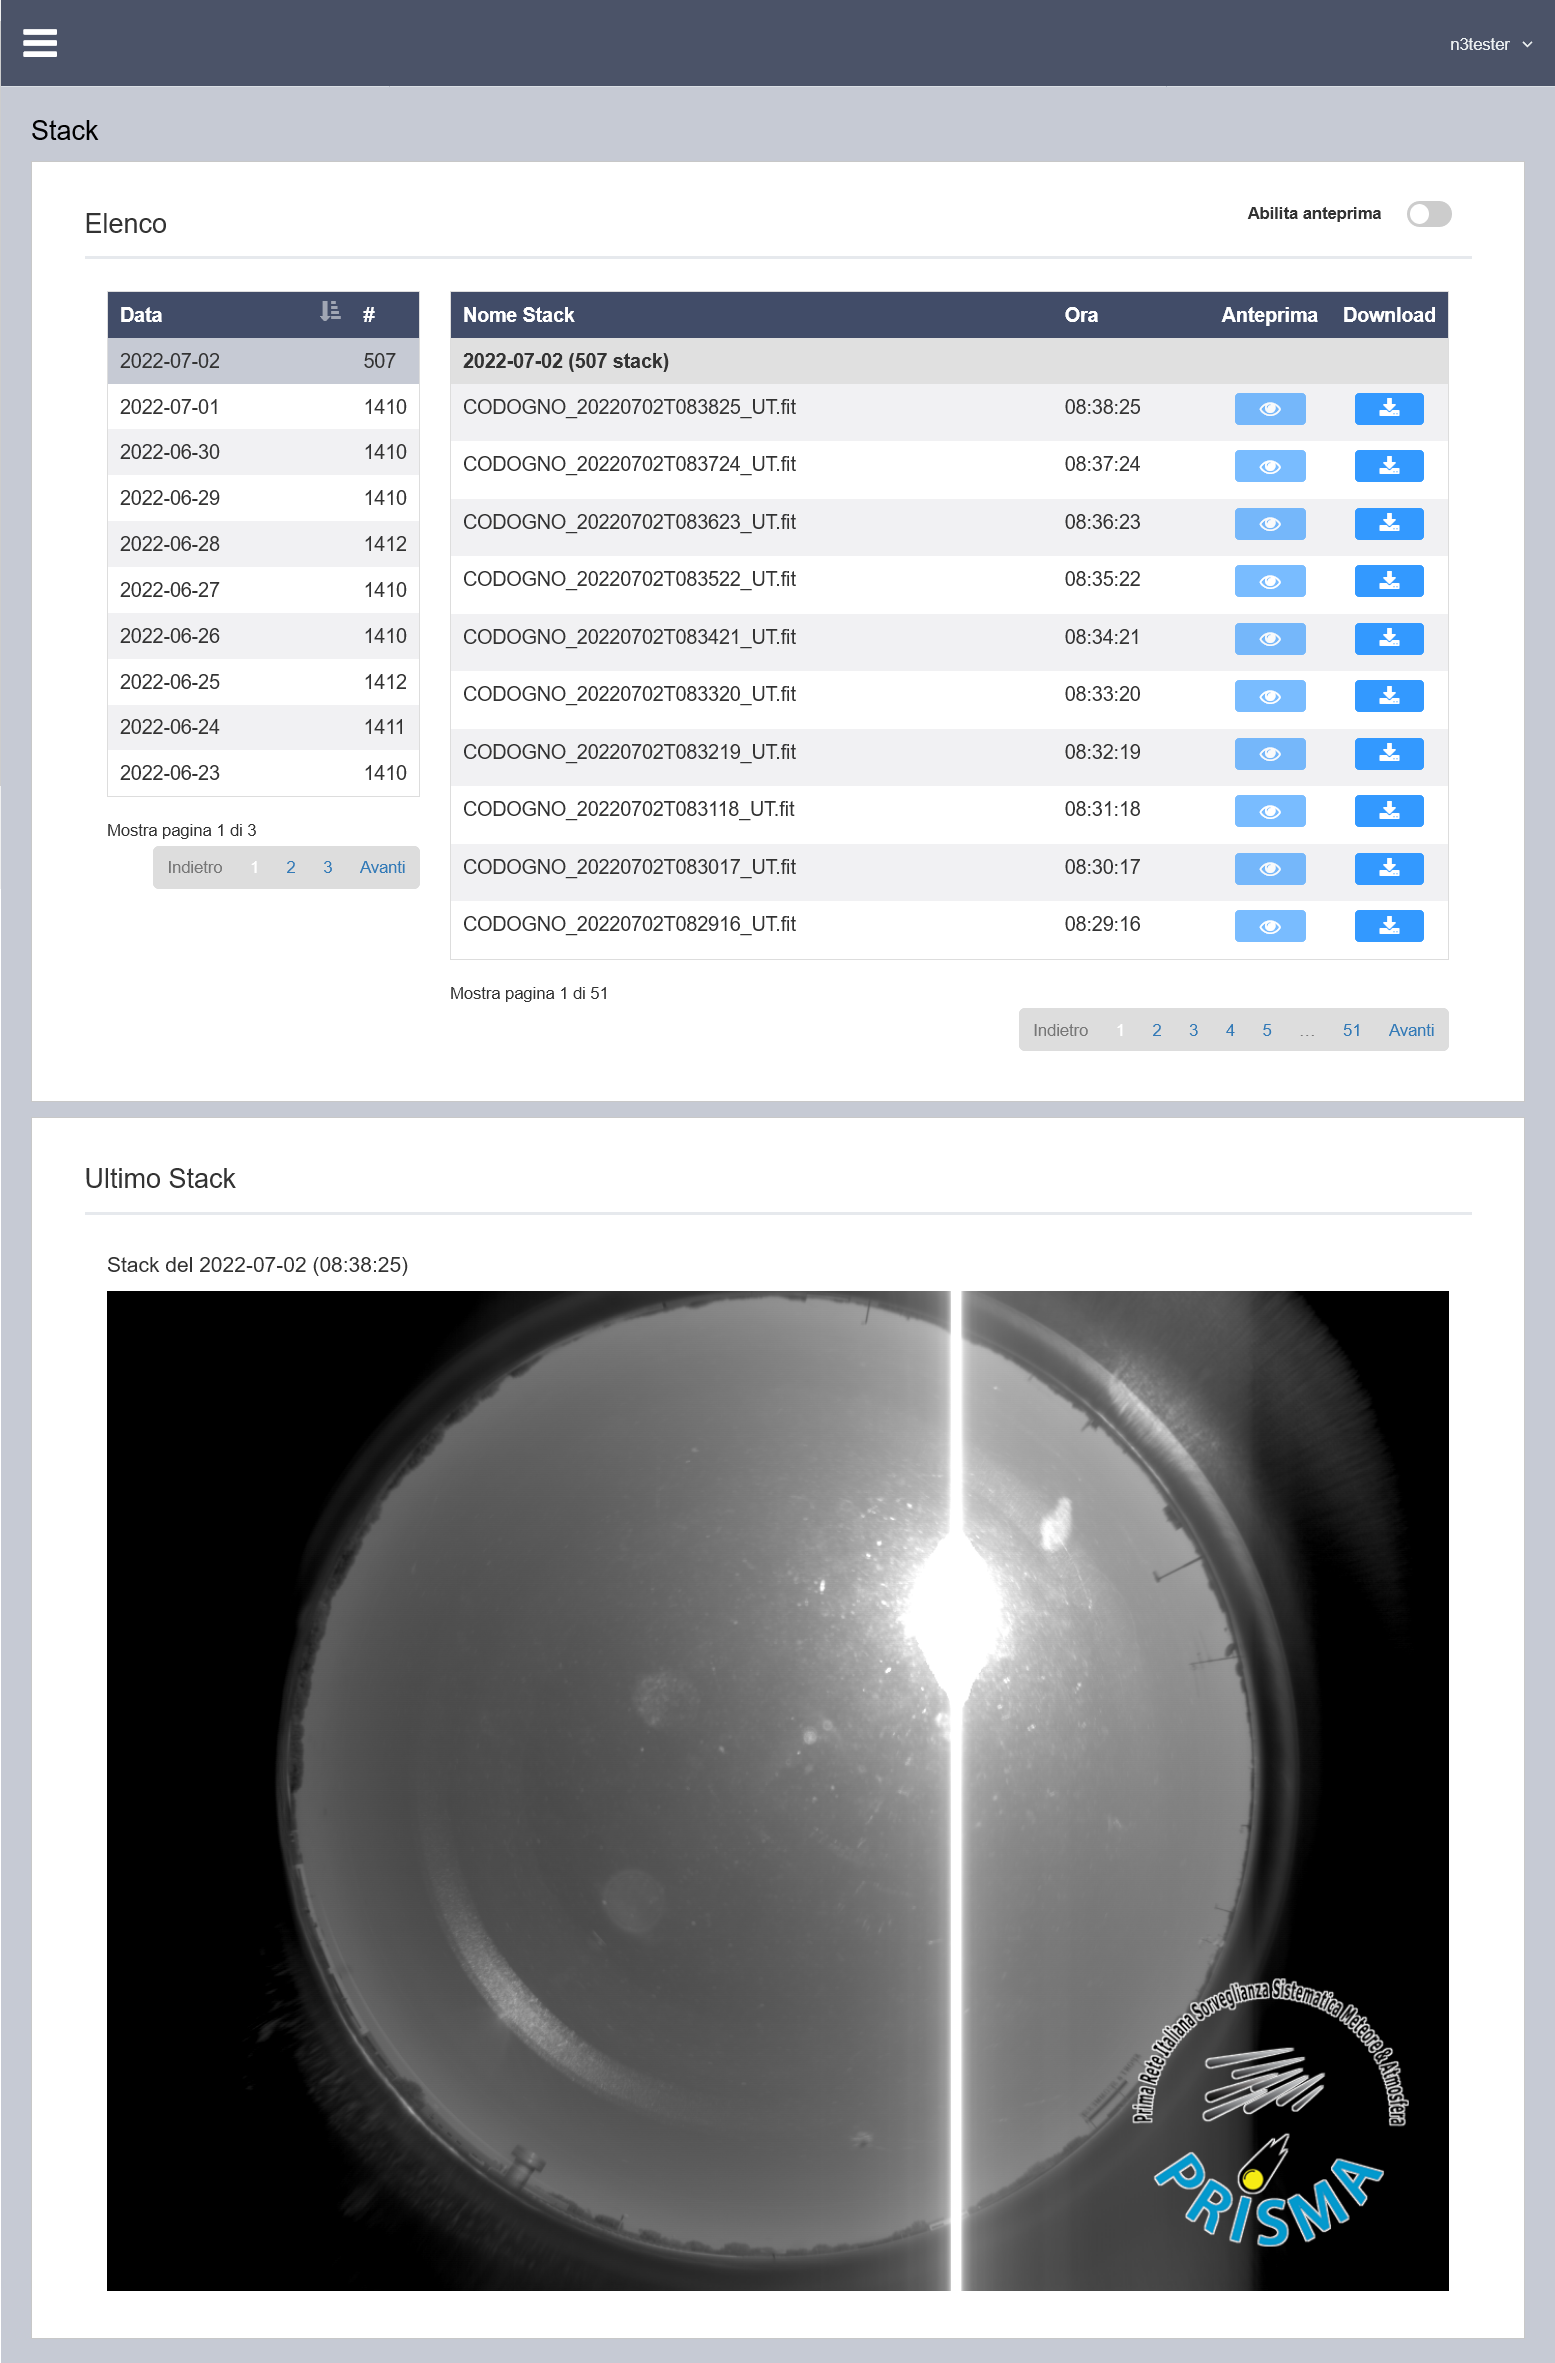
\includegraphics[width=\textwidth]{images/full-stacks.png}
    \caption{Sezione \emph{Stack}.}
    \label{fig:stack}
    \end{center}
\end{figure}